\chapter{2D Scattering}

  Here we address the scattering in two dimensions and compute the scattering length.

  The quantum scattering in 3 dimension is described in numerous textbooks and papers, so we omit explicitly referencing them here.

  Scattering in 2 dimensions follows the same approach as in 3D, with some subtle differences.
  We start with the Schrodinger equation in 2 dimensions, using atomic units:
  \begin{equation}\label{2DS1}
      \left(-\frac{1}{2}\nabla^2 + V(\mathbf{r})\right)\psi(\mathbf{r}) = E\psi(\mathbf{r})
  \end{equation}
  where $ \nabla $ is the 2D Laplacian: $ \nabla^2 = \frac{\partial^2 x}{\partial x^2} + \frac{\partial^2 y}{\partial y^2} $

  Switching to polar coordinates and using polar coordinates 2D Laplacian:
  \begin{equation}
      \left[-\frac{\partial^2}{\partial r^2} - \frac{1}{r}\frac{\partial}{\partial r} - \frac{1}{r^2}\frac{\partial^2}{\partial\phi^2} + V(r)\right]\psi(r,\phi) = 2E\ \psi(r,\phi)
  \end{equation}
  Using separation of variables: $ \psi(r,\phi) = F(r)T(\phi) $, we end up with 2 ordinary differential equations. We set $ k^2 = 2E $
  \begin{equation}
  \begin{split}
   & \frac{d^2F(r)}{d r^2} +\frac{1}{r}\frac{d F(r)}{d r} +(k^2 -  2V(r) - \frac{m^2}{r^2})F(r) = 0\\[.8em]
   & \frac{d^2 T(\phi)}{d \phi^2} + m^2 T(\phi) = 0
  \end{split}
  \end{equation}

  Note that the $ m $ is a quantum number, not the mass. 

  The function $ T(\phi) $ must be single valued and symmetric around the incident beam, taken to be around $ x $. In that case, m must be an integer, and solution must be symmetric along the x axis. Ergo the normalized angular function is:
  \begin{equation}
T(\phi) = \frac{1}{\sqrt{\pi}}e^{i m\phi}
\end{equation}
where m is an integer and we are using atomic units.

The radial equation $ F(r) $ is:
\begin{equation}\label{frr}
\frac{d^2 F}{dr^2} + \frac{1}{r}\frac{dF}{dr} + \left(k^2 - 2V(r) - \frac{m^2}{r^2}\right)F = 0
\end{equation}

Since scattering is a localized process so from the physics of the process and by examining the equation \eqref{frr},  we can identify 2 regions, the far away region and the scattering region.


\subsubsection{\textbf{Far away region, Incoming particle}}

For the regions far away from the scattering area where $ V(r) \rightarrow 0 $ we have a free space Schrodinger equation with $ k^2 = E $;
\begin{equation}\label{2DS1H}
\frac{d^2 F(r)}{dr^2} + \frac{1}{r}\frac{d Fr(r)}{dr} + \left(k^2 - \frac{m^2}{r^2}\right)F(r) = 0
\end{equation}
 
Here we have an incoming particle (or particle beam) with the uniform momentum $ \vec{p} $. So the general solution of the equation \eqref{frr} in the incoming plane wave: $  F(x) = e^{i\ kx} $, where $ k = \hbar\ p $.

The way to solve the equation \eqref{2DS1H} is to expand the incident wave in terms of Bessel function. This is the Partial-Wave Expansion method. We get:
\begin{equation}
    e^{i\ kx} = e^{i\ kr\cos\theta} = sum_{m=0}^{\infty}{\epsilon_m\i^m\cos(m\theta)R_m(kr)}
\end{equation}
where the most general form of $ R_m(kr) $ is the combination of cylindrical Bessel functions:
\begin{equation}\label{bss}
    R_m(kr) = A_mJ_m(kr) + B_mN_m(kr)
\end{equation}

We shall subsequently show the asymptotic form of the Bessel functions.

\subsubsection{\textbf{Far away region, Scattered particle}}

Here is still have the $ V(r) \rightarrow 0 $

In this region, the solution to the wave equation \eqref{frr} looks like the combination of the incoming plus the scattered outgoing wave.
\begin{equation}\label{free2D}
    R(r,\theta) = e^{ikx} + f(\theta)\frac{e^{ikr}}{\sqrt{r}}
\end{equation}

Now we can recognize the equation \eqref{frr} aa a 2D Helmholtz equation whose solution can be expressed as:
\begin{equation}\label{2DS2H}
\psi(\mathbf{r}) = \sum_{m}{C_mH_m^+(kr)e^{im\phi}}
\end{equation}
where $ H_m^+(kr) $ is the Hankel Function .
And for the $ r \rightarrow \infty $ we get approximate behaviour:
\begin{equation}\label{2DS2}
    H_m(kr) \xrightarrow[r \rightarrow \infty]{}\sqrt{\frac{2}{\pi k r}}exp\left[i\left(kr - \frac{(m + 1/2)\pi}{2}\right)\right] \sim e^{ikx} + f_m(\theta) \frac{e^{ikr}}{\sqrt{r}}
\end{equation}
where the term $ f(\theta) $ is the amplitude of the scattered wave relative to the incident wave. 
So in the remote region we have an incident plane wave propagating along the axis plus the scattered outgoing wave.

The scattering amplitude $ f_m $ is in the most general case, related to the phase shift $ \delta_m $ as $ f(\theta) \sim e^{i\delta(\theta)} - 1 $. \\
In the often used partial wave expansion the scattering amplitude and the phase shift are related as:
\begin{equation}
    f_m = \frac{e^{2i \delta_m}}{2ik} = \frac{e^{i\delta_m}\sin(\delta_m)}{k}
\end{equation}
In general the shape of the $ f(\theta) $ will depend on the symmetry of the system.

The actual $ f(\theta) $ is not observable however it is used to compute differential cross section
\begin{equation}
    \frac{d\sigma}{d\theta} = \frac{1}{k}\left|f(\theta)\right|^2
\end{equation}

\subsubsection{\textbf{Scattering region}}

In this case we consider the scattering area, where $ V(r) \neq 0 $. In this case we use the potential function $ V(R) $ obtained in chapter 2 and numerically solve the 2D Schrodinger equation. To obtain the phase shift we match the wave function in the scattering region to the wavefunction in the far away region and use the optical theorem.

In this regions the radial Schrodinger equation $ F(r) $ has the form:
\begin{equation}\label{frrSr}
\frac{d^2 F}{dr^2} + \frac{1}{r}\frac{dF}{dr} + \left(k^2 - 2V(r) - \frac{m^2}{r^2}\right)F = 0
\end{equation}


\subsubsection{Scattering Process}

Now we expand:
\begin{equation}\label{expE}
e^{ikx} = e^{ikr\cos\theta} = \sum_m{\epsilon_m i^m \cos(m\theta)J_m(kr)}
\end{equation}
where $\epsilon_m = 2 $ for $ m \neq 0 $ and $ \epsilon_0 = 1 $.

Note: This looks very similar to the 3D case. The main difference is that in 2D case, the solution is a sum of cylindrical Bessel functions $ J_m(kr) $ and $ N_m(kr) $.
In the 3D case, the solution is the sum of the spherical Bessel functions.

Using asymptotic expressions for $ r \rightarrow \infty 0$:
\begin{equation}\label{}
\begin{split}
& J_m(kr) \xrightarrow{r \rightarrow \infty}  = \sqrt{\frac{2}{\pi k r}}\cos\left(kr - \frac{m\pi}{2} - \frac{\pi}{4}\right) \\[.7em]
& N_m(kr) \xrightarrow{r \rightarrow \infty}  = \sqrt{\frac{2}{\pi k r}}\sin\left(kr - \frac{m\pi}{2} - \frac{\pi}{4}\right)
\end{split}
\end{equation}
The most general solution of the radial part is in the absence of potential is:
\begin{equation}\label{bigRBsl}
R(r) = A_mJ_m(kr) + B_mN_m(kr) 
\end{equation}
For $ r \rightarrow\infty $ the \eqref{bigRBsl} has asymptotic form
\begin{equation}\label{asympR}
R(r) = A_m\frac{1}{\sqrt{kr}}\cos\left[kr-\pi\frac{m + 1/2}{2} + \delta_m\right]
\end{equation}
Now equating equations \eqref{asympR} and and using \eqref{expE},\eqref{asymp2} we obtain:
\begin{equation}\label{asymR2}
\begin{split}
& \sum_m{\epsilon_m i^m\sqrt{\frac{2}{\pi kr}}\cos(m\theta)\cos\left[kr-\pi\frac{m + 1/2}{2}\right]} + f(\theta)\frac{e^{ikr}}{\sqrt{r}} = \\[.7em]
& \sum_m{A_m\frac{1}{\sqrt{kr}}\cos\left[kr-\pi\frac{m + 1/2}{2} + \delta_m\right]\cos(m\theta)}
\end{split}
\end{equation}
Now this can be rewritten as:
\begin{equation}\label{asyR3}
\begin{split}
& \sum_m{\epsilon_m i^m \sqrt{\frac{2\cos(m\theta)}{\pi kr}}\left[e^{i\left(kr-\pi\frac{m + 1/2}{2}\right)} + e^{-i\left(kr-\pi\frac{m + 1/2}{2}\right)}\right]}
+ f(\theta)\frac{e^{ikr}}{\sqrt{r}} = \\[.7em]
& \sum_m{A_m\frac{\cos(m\theta)}{\sqrt{kr}}\left[e^{i\left(kr-\pi\frac{m + 1/2}{2} + \delta_m\right)} + e^{-i\left(kr-\pi\frac{m + 1/2}{2} + \delta_m\right)}\right]}
\end{split}
\end{equation}
Now coefficients with $ e^{ikr} $ and $ e^{-ikr} $ must be equal. After some algebra and following \cite{2DScatter2} we get:
\begin{equation}\label{AandDelta}
A_m = 2\epsilon_m \frac{i^m}{\sqrt{2\pi k}}e^{i\delta_m}
\end{equation}
So the scattering amplitude is:
\begin{equation}
f(\theta) = \sqrt{\frac{1}{2\pi i k}}\sum_{m=0}^{\infty}{\epsilon_m\cos(m\theta)\left[e^{2i\delta_m}-1\right]}
\end{equation}

So far, this is a general formula applicable to any kind of process.

\subsubsection{Scattering Length for the Hydrogen Molecular Ion in 2D}

For the actual calculation we first start from the form of the radial wave function for the scattered free particle
\begin{equation}\label{remoteWave2}
    R_m(r) = \cos \delta_m(kr) J_m(kr) + \sin \delta_m(kr) N_m(kr)
\end{equation}
 
Now we need to match the solution in the scattering region, which is obtain numerically with the analytical solution above for the remote region. We also need to match the derivatives. The practical way to do it is to use the logarithmic derivative. We increase the value of R until we observer the convergence of $ \delta $ to some final value.

The other practical method and arguably more practical is to follow the Calogero's approach \cite{Calogero}.
From the equation \eqref{remoteWave2}, the $ \delta_m(r) $ satisfies an differential equation:
\begin{equation}\label{delta_eq}
    \frac{d\delta_m}{dr} = -\frac{V(r)}{k}\left[\cos \delta_m(kr) J_m(kr) + \sin \delta_m(kr) N_m(kr)\right]^2
\end{equation}

Now to find the value of $ \delta $ we integrate from some starting point $ r $ to obtain:
\begin{equation}\label{delta_r}
    \delta_m = \lim_{r \rightarrow \infty}\delta_m(r) 
\end{equation}

Following the \cite{Dalgarno1953} we then proceed to compute the scattering length. We choose the 'room' temperature range.

The Mathematica code that computes the phase shift and the cross section  is in appendix E.

The following graphs show the phase shift and the scattering length for the 2D H2 ion at 'room' temperatures.

\begin{figure}
 \captionsetup{type=figure}
    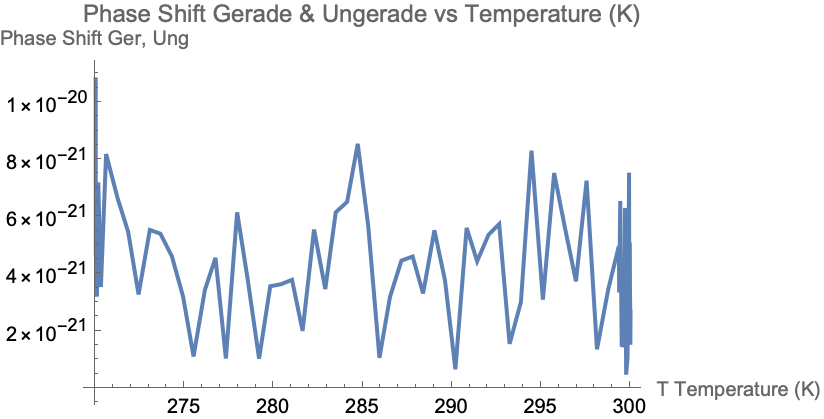
\includegraphics{PhaseShift-Ger-Ung.png}
  \caption{Phase Shift, $ \delta_G - \delta_U $ }
    \label{phaseShift2D}
\end{figure}


\begin{figure}
 \captionsetup{type=figure}
    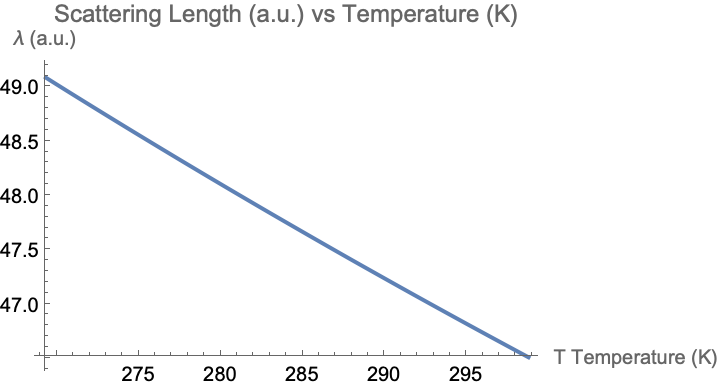
\includegraphics{Scatterring-length.png}
  \caption{Scattering Length}
    \label{scatterLen}
\end{figure}
